\documentclass{article}
\usepackage{amsmath}
\usepackage[english]{babel}
\usepackage{graphicx}
\usepackage{subcaption}
\usepackage{listings}
\usepackage{geometry}
\usepackage{titling}
\usepackage{matlab-prettifier}
\usepackage{pythonhighlight}
\usepackage{gensymb}
\usepackage{mathtools}
\usepackage{hyperref}
\usepackage{authblk}
\geometry{
    left=30mm,
    right=30mm,
    top=20mm,
    bottom=20mm
}
%\setlength{\droptitle}{-10em}

\title{Computer Vision Programming Homework \#1}
\author{2022094093 Kim Dohoon}
\affil{Department of Data Science, Major in Data Science}

\begin{document}
\maketitle

\section{Original Image}
First we need to load original images.
\begin{figure}[!ht]
    \centering
    \begin{subfigure}{0.356\textwidth}
        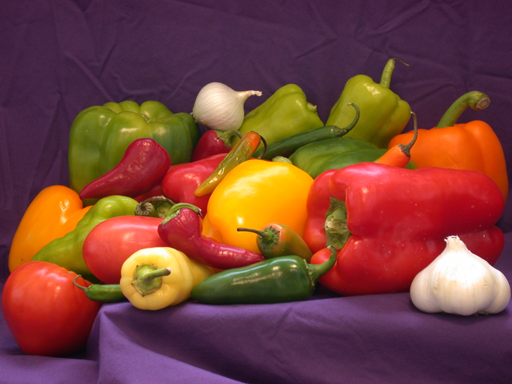
\includegraphics[width=\textwidth]{./fig/peppers.png}
        \caption{peppers}
    \end{subfigure}
    \begin{subfigure}{0.267\textwidth}
        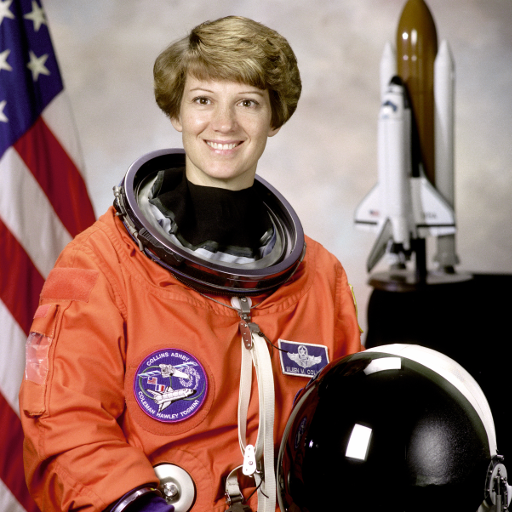
\includegraphics[width=\textwidth]{./fig/astronaut.png}
        \caption{astronaut}
    \end{subfigure}
    \begin{subfigure}{0.2\textwidth}
        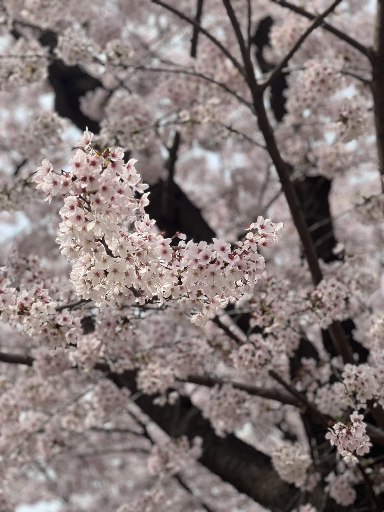
\includegraphics[width=\textwidth]{./fig/cb.png}
        \caption{Own image}
    \end{subfigure}
    \caption{Images before transform}
\end{figure}

Also, let $(x, y)$ be an original point, and $(x', y')$ be a transformed point.
$$f : (x, y) \rightarrow (x', y')$$


\newpage
\section{Projective Image Transformation}

\subsection{Scaling}
Scale transform is defined as below. Translation is skipped.  

$$ \begin{bmatrix}
x' \\ y' \\ 1
\end{bmatrix}
=
\begin{bmatrix}
s & 0 & 0 \\
0 & s & 0 \\
0 & 0 & 1
\end{bmatrix}
\begin{bmatrix}
x \\ y \\ 1
\end{bmatrix} $$
where $s$ is scaling factor, and degree of freedom is 1. 
If we want to scale $x$ and $y$ differently, we can just use $s_x$ and $s_y$. 
Then degree of freedom is 2.

\begin{figure}[!ht]
    \centering
    \begin{subfigure}{0.356\textwidth}
        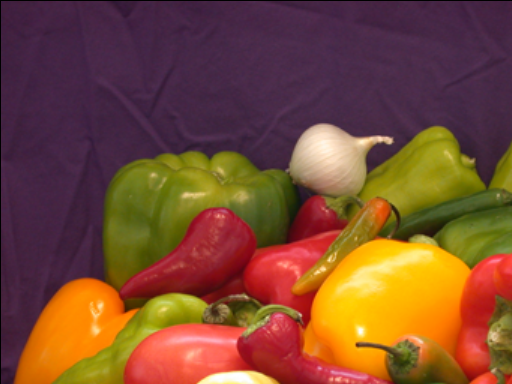
\includegraphics[width=\textwidth]{./fig/scaling_peppers.png}
        \caption{peppers, Matlab}
    \end{subfigure}
    \begin{subfigure}{0.267\textwidth}
        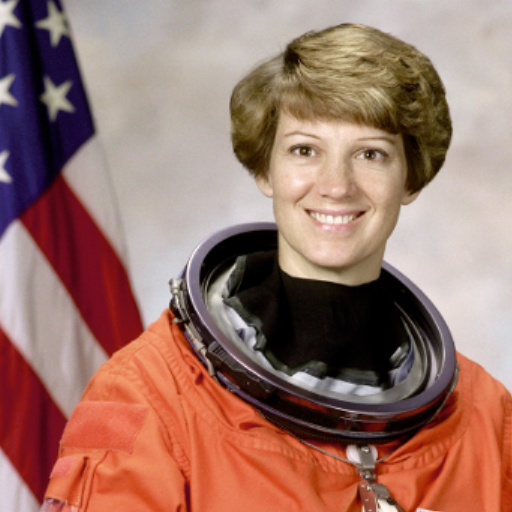
\includegraphics[width=\textwidth]{./fig/scaling_astronaut.png}
        \caption{astronaut, Python}
    \end{subfigure}
    \begin{subfigure}{0.2\textwidth}
        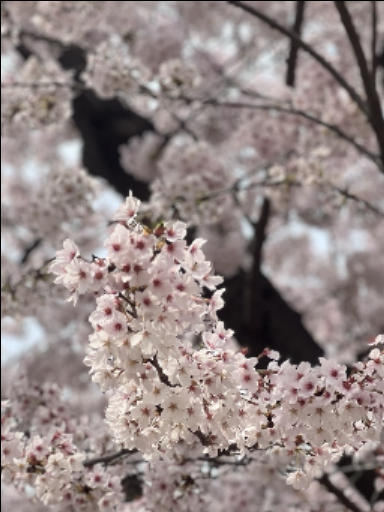
\includegraphics[width=\textwidth]{./fig/scaling_cb.png}
        \caption{Own image}
    \end{subfigure}
    \caption{Scaling transform}
\end{figure}
\subsection{Rotation}
Rotation transform is defined as below. Translation is skipped.
$$
\begin{bmatrix}
x' \\ y' \\ 1
\end{bmatrix}
=
\begin{bmatrix}
\cos\theta & -\sin\theta & 0 \\
\sin\theta & \cos\theta & 0 \\
0 & 0 & 1
\end{bmatrix}
\begin{bmatrix}
x \\ y \\ 1
\end{bmatrix}
$$
where $\theta$ is angle to rotate. Since only $\theta$ determines the matrix, degree of freedom is 1.

\begin{figure}[!ht]
    \centering
    \begin{subfigure}{0.356\textwidth}
        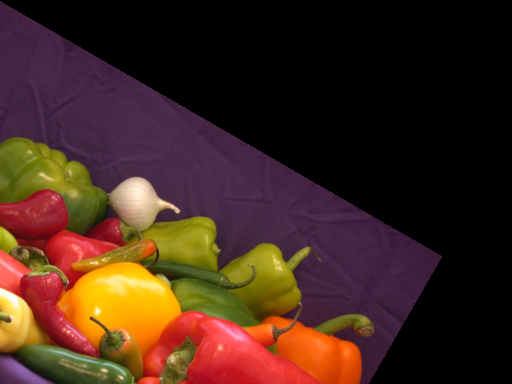
\includegraphics[width=\textwidth]{./fig/rotation_peppers.png}
        \caption{peppers, Matlab}
    \end{subfigure}
    \begin{subfigure}{0.267\textwidth}
        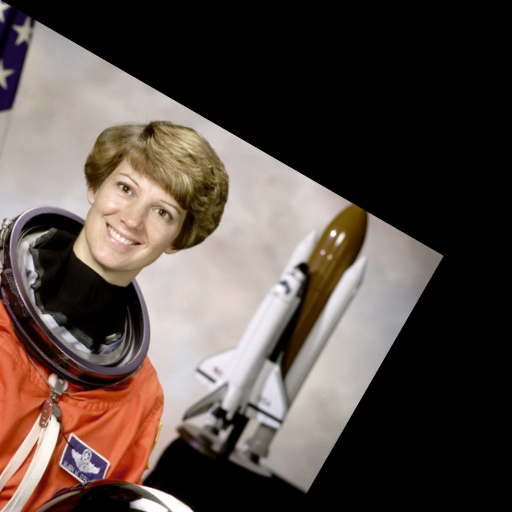
\includegraphics[width=\textwidth]{./fig/rotation_astronaut.png}
        \caption{astronaut, Python}
    \end{subfigure}
    \begin{subfigure}{0.2\textwidth}
        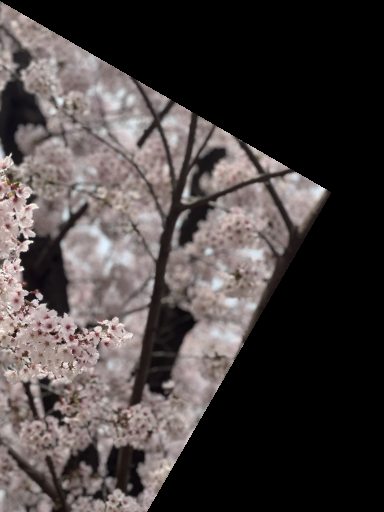
\includegraphics[width=\textwidth]{./fig/rotation_cb.png}
        \caption{Own image}
    \end{subfigure}
    \caption{Rotation transform}
\end{figure}

\newpage
\subsection{Similarity}
Similarity transform means scaling and rotating together. So, it is defined as below. Translation is skipped.
$$
\begin{bmatrix}
x' \\ y' \\ 1
\end{bmatrix}
=
s
\begin{bmatrix}
\cos\theta & -\sin\theta & 0 \\
\sin\theta & \cos\theta & 0 \\
0 & 0 & 1
\end{bmatrix}
\begin{bmatrix}
x \\ y \\ 1
\end{bmatrix}
\\
= \begin{bmatrix}
s\cdot \cos\theta & -s\cdot \sin\theta & 0 \\
s\cdot \sin\theta & s\cdot \cos\theta & 0 \\
0 & 0 & 1
\end{bmatrix}
\begin{bmatrix}
x \\ y \\ 1
\end{bmatrix}
$$
where $s$ is scaling factor and $\theta$ is angle to rotate. So degree of freedom is 2.

\begin{figure}[!ht]
    \centering
    \begin{subfigure}{0.356\textwidth}
        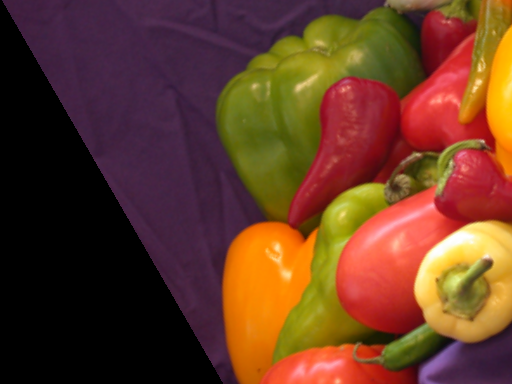
\includegraphics[width=\textwidth]{./fig/similarity_peppers.png}
        \caption{peppers, Matlab}
    \end{subfigure}
    \begin{subfigure}{0.267\textwidth}
        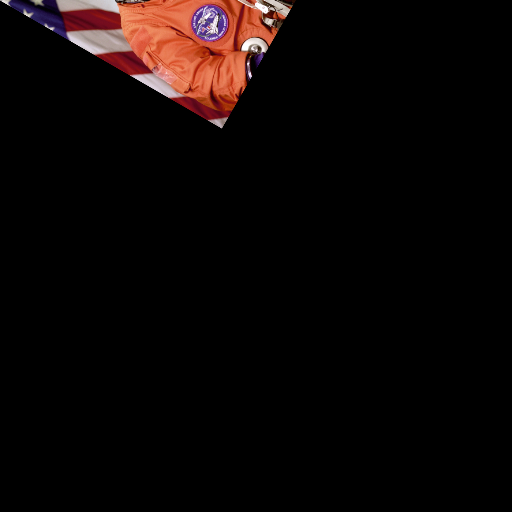
\includegraphics[width=\textwidth]{./fig/similarity_astronaut.png}
        \caption{astronaut, Python}
    \end{subfigure}
    \begin{subfigure}{0.2\textwidth}
        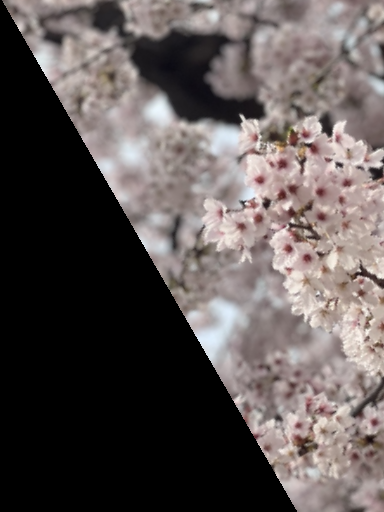
\includegraphics[width=\textwidth]{./fig/similarity_cb.png}
        \caption{Own image}
    \end{subfigure}
    \caption{Similarity transform}
\end{figure}

\subsection{Affine}
Without changing last row vector (which is $\begin{bmatrix}0 & 0 & 1\end{bmatrix}$), Affine transform is the generalized form.
Now we have scaling, rotating, and translating.  

$$ \begin{bmatrix}
    x' \\ y' \\ 1
    \end{bmatrix}
    =
    \begin{bmatrix}
    a & b & c \\
    d & e & f \\
    0 & 0 & 1
    \end{bmatrix}
    \begin{bmatrix}
    x \\ y \\ 1
\end{bmatrix} $$
Degree of freedom is 6 due to the variables from $a$ to $f$.
Here, I used this matrix.
$$ 
\begin{bmatrix}
    2 & 0.2 & -100 \\
    0.33 & 1 & 50 \\
    0 & 0 & 1
\end{bmatrix} 
$$

\begin{figure}[!ht]
    \centering
    \begin{subfigure}{0.356\textwidth}
        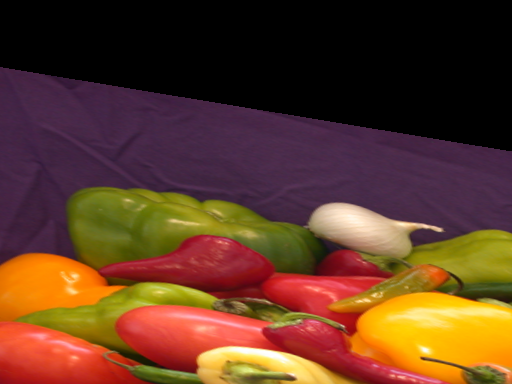
\includegraphics[width=\textwidth]{./fig/affine_peppers.png}
        \caption{peppers, Matlab}
    \end{subfigure}
    \begin{subfigure}{0.267\textwidth}
        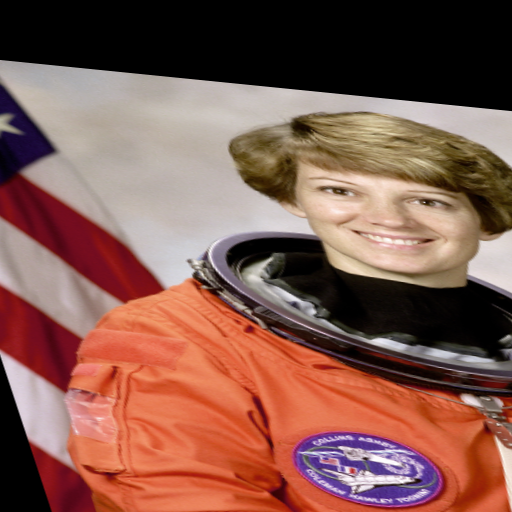
\includegraphics[width=\textwidth]{./fig/affine_astronaut.png}
        \caption{astronaut, Python}
    \end{subfigure}
    \begin{subfigure}{0.2\textwidth}
        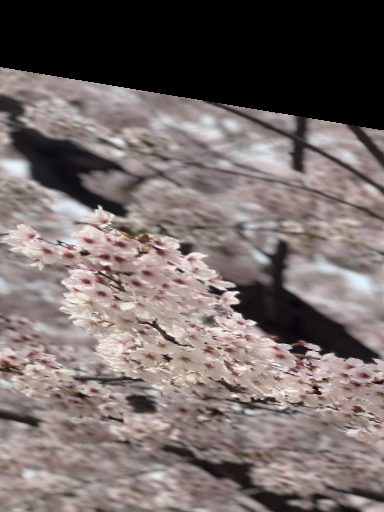
\includegraphics[width=\textwidth]{./fig/affine_cb.png}
        \caption{Own image}
    \end{subfigure}
    \caption{Affine transform}
\end{figure}

\newpage
\subsection{Projective}
Without changing last item (row 3, column 3 as 1), Projective transform is the most generalized form.
Now we have scaling, rotating, and translating.  

$$ \begin{bmatrix}
    x' \\ y' \\ 1
    \end{bmatrix}
    =
    \begin{bmatrix}
    a & b & c \\
    d & e & f \\
    g & h & 1
    \end{bmatrix}
    \begin{bmatrix}
    x \\ y \\ 1
\end{bmatrix} $$
Degree of freedom is 6 due to the variables from $a$ to $f$.
Here, I used this matrix.
$$ 
\begin{bmatrix}
    1 & -0.1 & 50 \\
    0.2 & 0.07 & 30 \\
    0.005 & -0.005 & 1
\end{bmatrix} 
$$

\begin{figure}[!ht]
    \centering
    \begin{subfigure}{0.356\textwidth}
        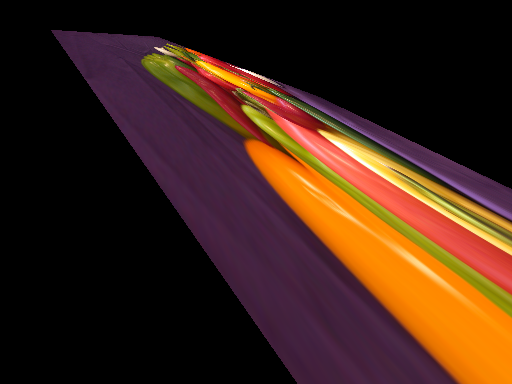
\includegraphics[width=\textwidth]{./fig/projective_peppers.png}
        \caption{peppers, Matlab}
    \end{subfigure}
    \begin{subfigure}{0.267\textwidth}
        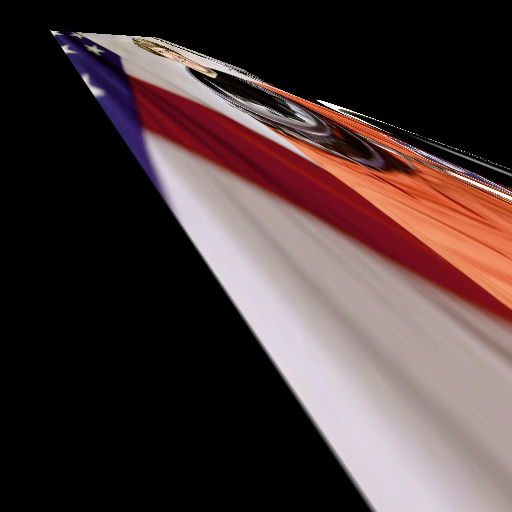
\includegraphics[width=\textwidth]{./fig/projective_astronaut.png}
        \caption{astronaut, Python}
    \end{subfigure}
    \begin{subfigure}{0.2\textwidth}
        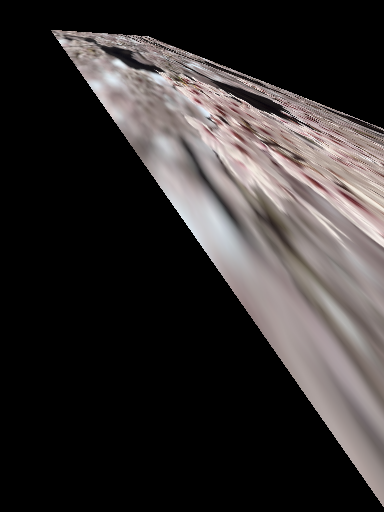
\includegraphics[width=\textwidth]{./fig/projective_cb.png}
        \caption{Own image}
    \end{subfigure}
    \caption{Projective transform}
\end{figure}

\newpage
\section{Color Space}
\subsection{RGB}
To display RGB channel of image separately, we can just index them.

\begin{figure}[h]
    \centering
    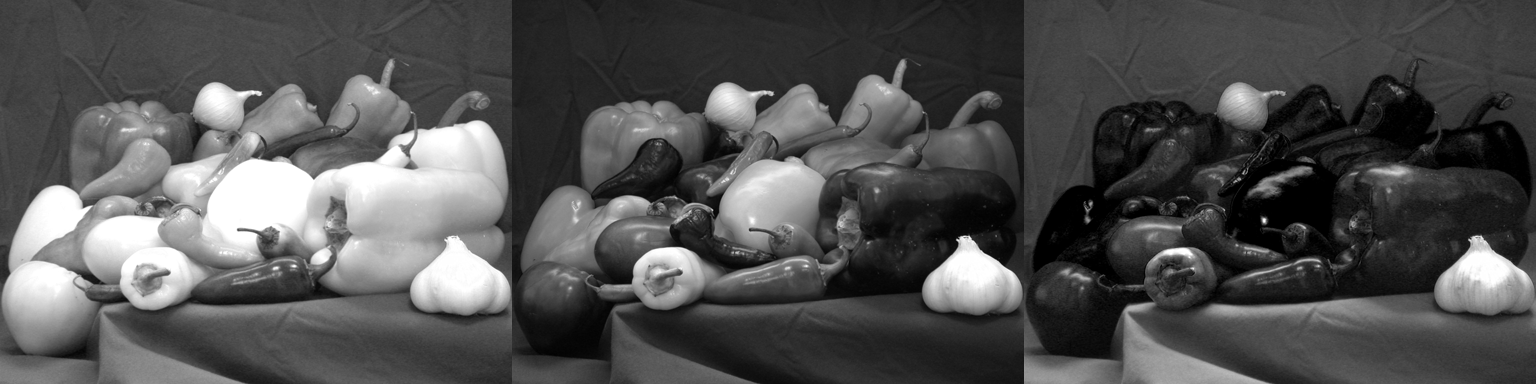
\includegraphics[width=.4\textwidth]{fig/RGB_peppers.png}\\
    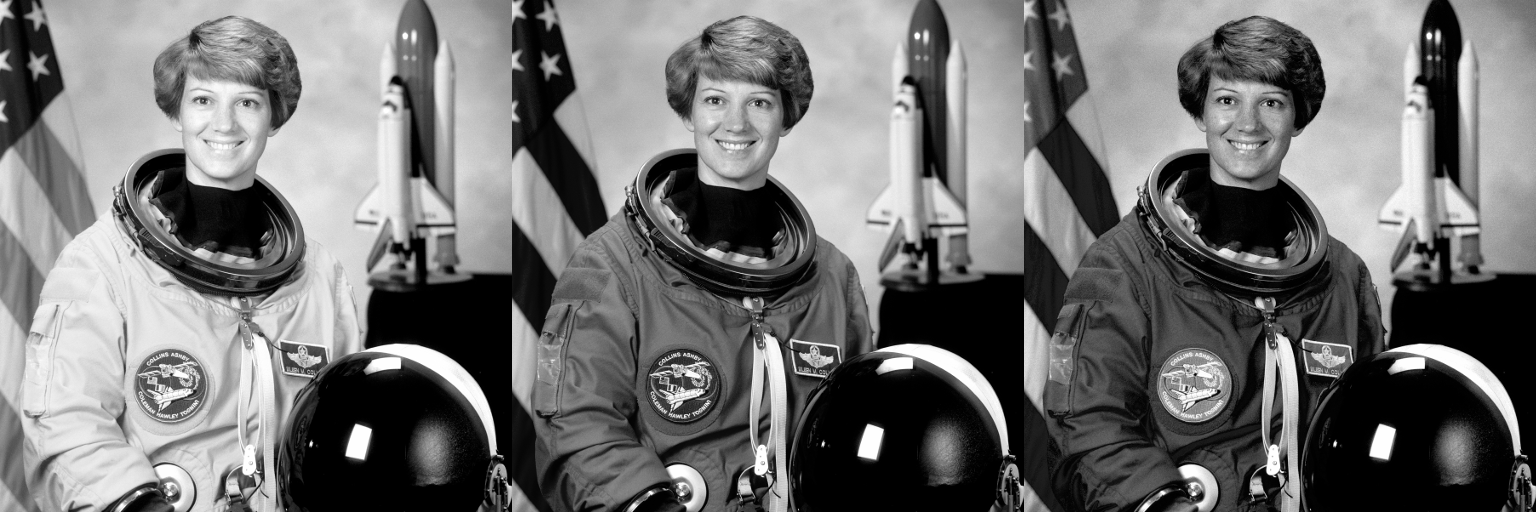
\includegraphics[width=.4\textwidth]{fig/RGB_astronaut.png}\\
    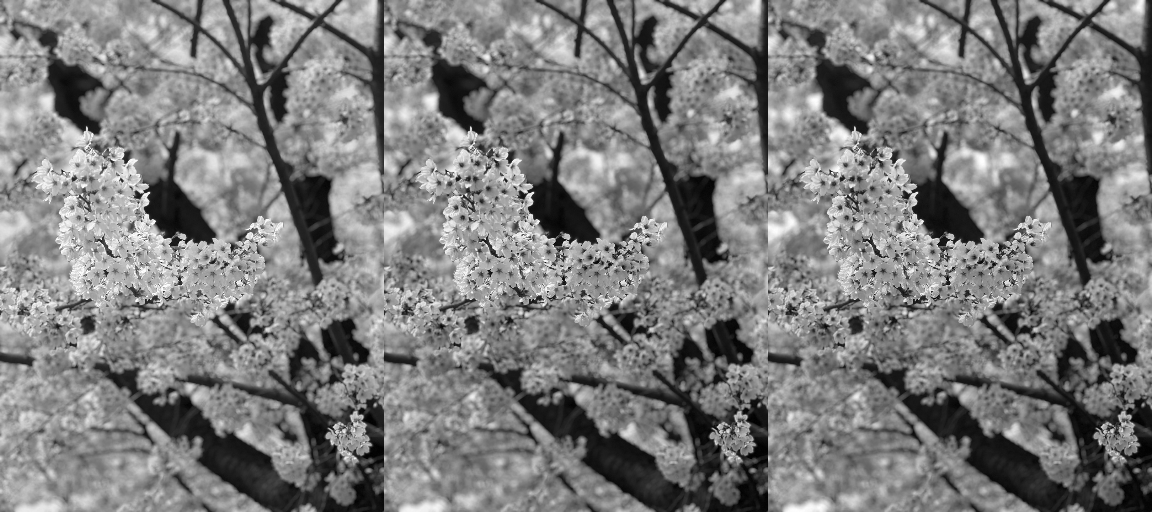
\includegraphics[width=.4\textwidth]{fig/RGB_cb.png}
    \caption{R, G, B}
\end{figure}

\subsection{YCbCr}
To convert color space from RGB to YCbCr, perform this linear transformation.
$$
\begin{bmatrix}
    Y \\ C_B \\ C_R
\end{bmatrix}
=
\frac{1}{256}
\begin{bmatrix}
    77 & 150 & 29 \\
    -43 & -84 & 127 \\
    127 & -106 & -21
\end{bmatrix}
\begin{bmatrix}
    R \\ G \\ B
\end{bmatrix}
+
\begin{bmatrix}
    0 \\ 128 \\ 128
\end{bmatrix}
$$ 
where $(R, G, B)$ is the RGB value at some pixel, $Y$ is luminance, $C_B$ is blue color and $C_R$ is red color.

\begin{figure}[h]
    \centering
    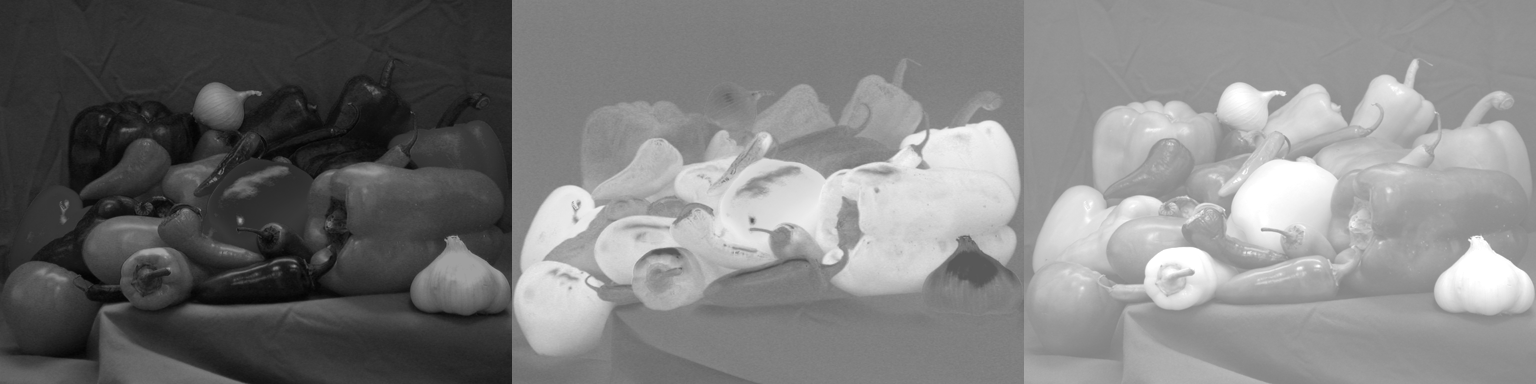
\includegraphics[width=.4\textwidth]{fig/YCbCr_peppers.png}\\
    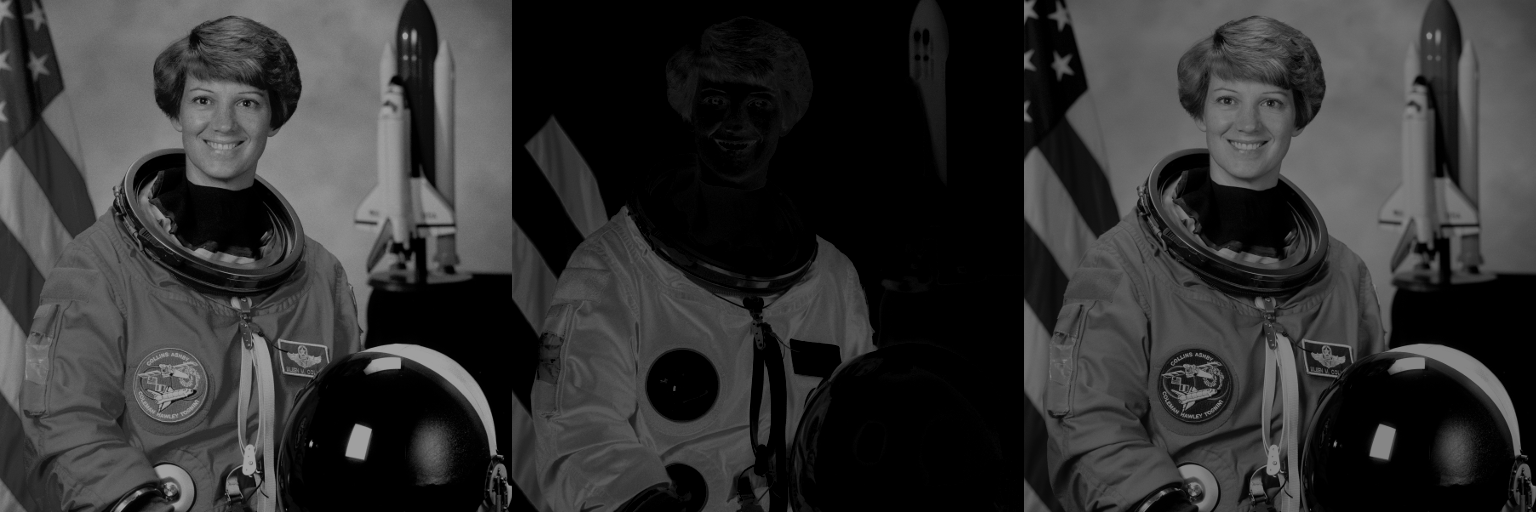
\includegraphics[width=.4\textwidth]{fig/YCbCr_astronaut.png}\\
    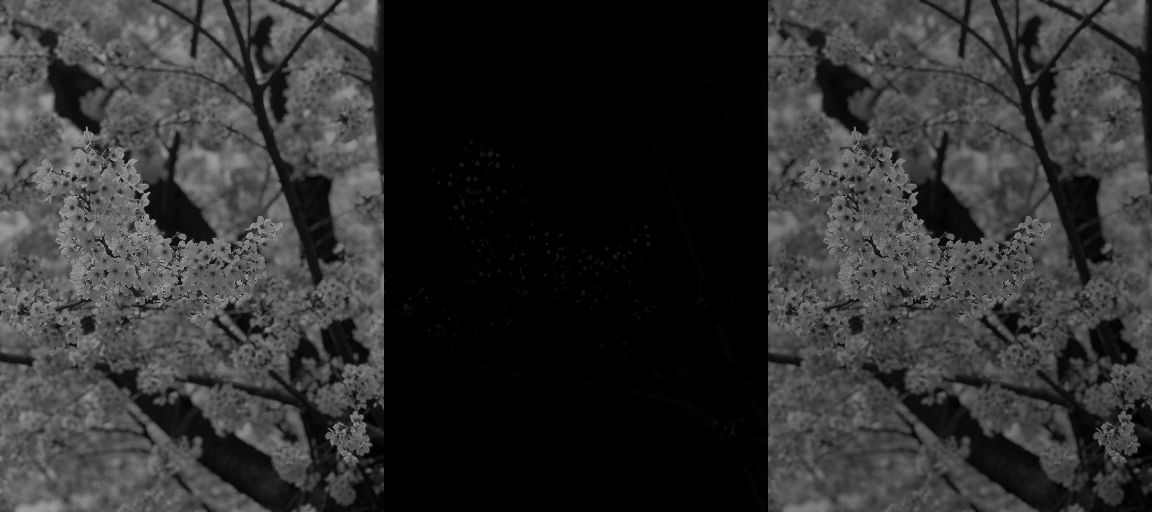
\includegraphics[width=.4\textwidth]{fig/YCbCr_cb.png}
    \caption{Y, Cb, Cr}
\end{figure}


\newpage
\subsection{HSI}
To convert color space from RGB to HSI, we can use this formula.

\begin{gather*}
    H' = \cos^{-1} \Biggl \{ \frac{2R_N - G_N - B_N}{2\sqrt{(R_N-G_N)^2 + (R_N-B_N)(G_N-B_N)}} \Biggl \} \\
    H = 
    \begin{dcases*}
    \frac{1}{2\pi}H' & if $R_N \leq G_N$ \\
    1 - \frac{1}{2\pi}H' & if $R_N > G_N$
    \end{dcases*} 
    \\
    S = 1 - \frac{\min(R_N,G_N,B_N)}{I}  \\
    I = \frac{1}{3} (R_N + G_N + B_N)
\end{gather*}
H is the color, S is the strength of color, and I is the strength of light.   
Also, Hue is not defined where Intensity is 0.


\begin{figure}[h]
    \centering
    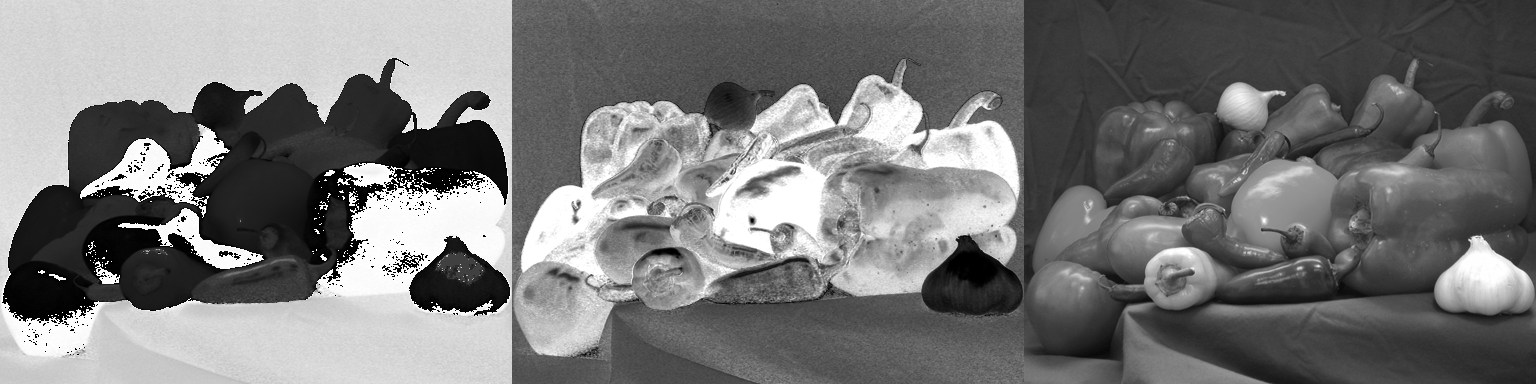
\includegraphics[width=.4\textwidth]{fig/HSI_peppers.png}  \\
    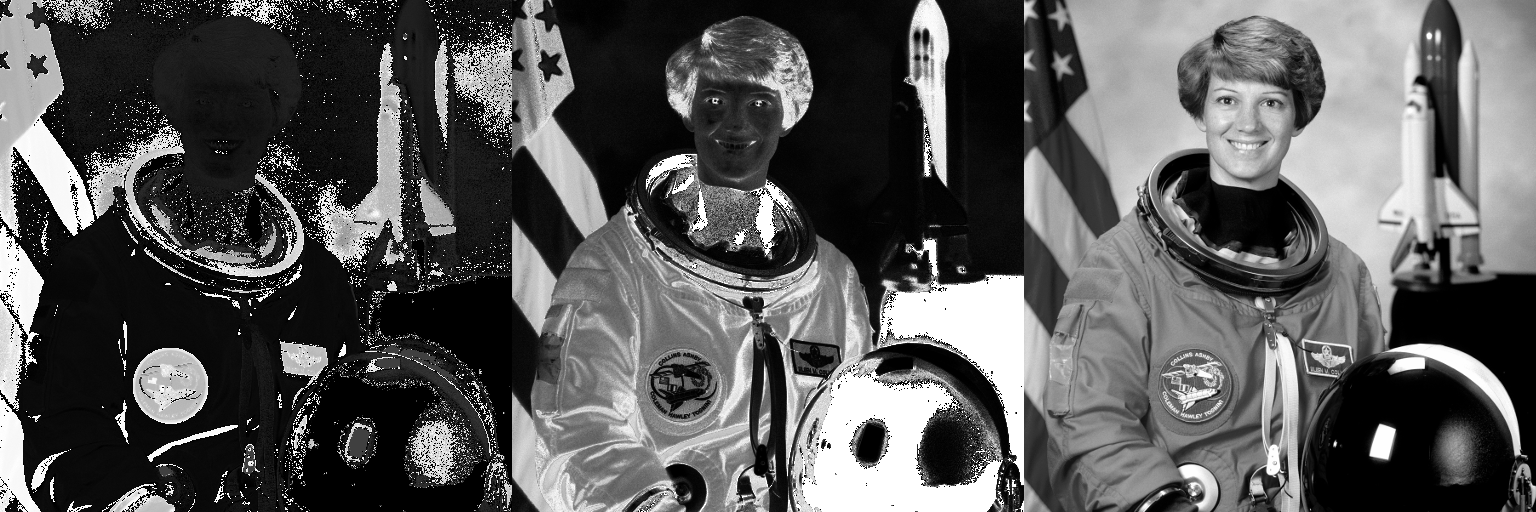
\includegraphics[width=.4\textwidth]{fig/HSI_astronaut.png}  \\
    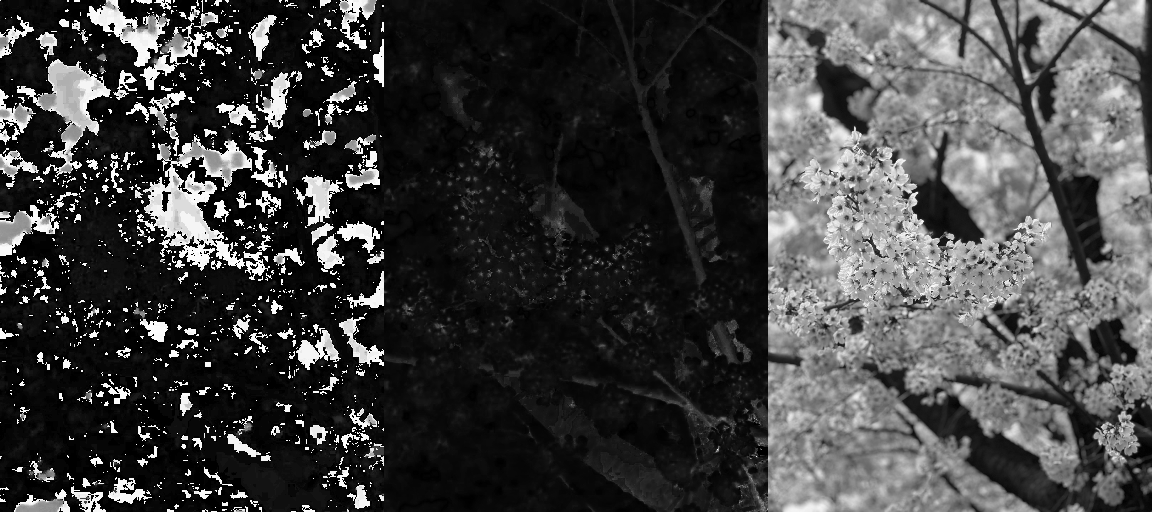
\includegraphics[width=.4\textwidth]{fig/HSI_cb.png}
    \caption{H, S, I}
\end{figure}

\subsection{Comparison}
$RGB$, $YCbCr$, and $HSI$ are color model to express image, but they are different, as above.
RGB is the most simple model, to express image.
YCbCr is useful due to is compressibility. 
HSI is useful to modify color information, since intensity is separated to color. H plot is very spotted, since it contains the whole color information.

\newpage
\subsection{Modifying Image}
After multipling $2\pi$ to convert to radian, Transformation from HSI to RGB follows as;  

\begin{gather*}
    C_1 = I(1-S)  \\
    C_2 = I \Big[ 1 + \frac{S \cos H}{\cos(\pi/3 - H)} \Big]  \\
    C_3 = 3I - (C_1 + C_2) \\
    (R, G, B) =
    \begin{dcases*}
        (C_3, C_1, C_2) & if $0 \leq H < \frac{2\pi}{3}$ \\
        (C_2, C_3, C_1) & if $\frac{2\pi}{3} \leq H < \frac{4\pi}{3}$ \\
        (C_1, C_2, C_3) & if $\frac{4\pi}{3} \leq H < 2\pi$
    \end{dcases*}
\end{gather*}
I added 16/255 to Saturation, and 16/255 to Intensity. 

\begin{figure}[!ht]
    \centering
    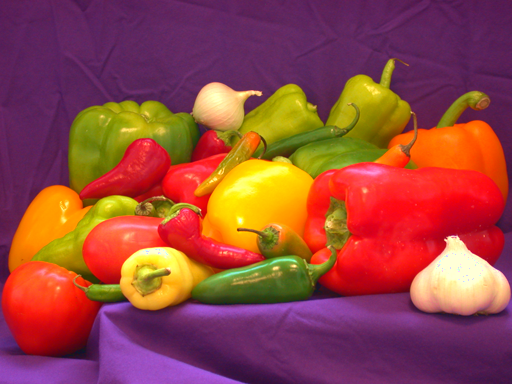
\includegraphics[width=.356\textwidth]{fig/HSI2RGB_peppers.png}
    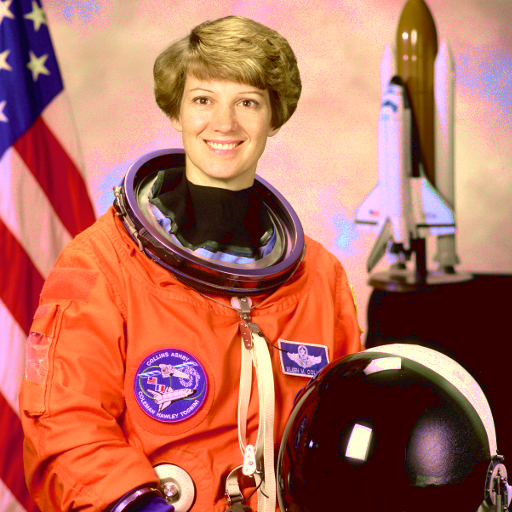
\includegraphics[width=.267\textwidth]{fig/HSI2RGB_astronaut.png}
    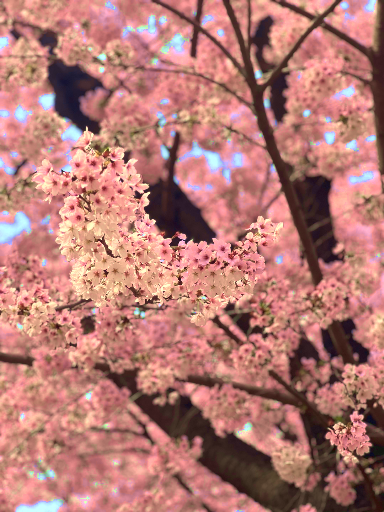
\includegraphics[width=.2\textwidth]{fig/HSI2RGB_cb.png}
    \caption{Modified HSI to RGB}
\end{figure}


\section*{Appendix}
All codes and images are at \url{https://github.com/kdh-yu/ComputerVision/tree/main/HW_1}

\end{document}